\documentclass[letterpaper,10pt]{article}
% use UTF8 encoding
\usepackage[utf8]{inputenc}
% use KoTeX package for Korean 
\usepackage[english]{babel}
\usepackage{multirow}
\usepackage{array}
\usepackage[dvipsnames]{xcolor}
\usepackage{kotex}
\usepackage{adjustbox}
\usepackage{tabularx} % extra features for tabular environment
\usepackage{amsmath}  % improve math presentation
\usepackage{amssymb}
\usepackage{graphicx} % takes care of graphic including machinery
\usepackage[margin=1in,letterpaper]{geometry} % decreases margins
\usepackage{cite} % takes care of citations
\usepackage[final]{hyperref} % adds hyper links inside the generated pdf file
\usepackage{minted}
\hypersetup{
	colorlinks=true,       % false: boxed links; true: colored links
	linkcolor=blue,        % color of internal links
	citecolor=blue,        % color of links to bibliography
	filecolor=magenta,     % color of file links
	urlcolor=blue         
}
\usepackage{blindtext}
%++++++++++++++++++++++++++++++++++++++++


\setlength{\parskip}{1.0em}
\renewcommand{\baselinestretch}{1.25}
\begin{document}
	
	\title{2. $n$차원 입력의 Percentron Learning}
	\author{2019920017 컴퓨터과학부 김정현}
	\date{2021/10/06까지}
	\maketitle
	
	\section{구현 방법 소개}
	
	\subsection{퍼셉트론의 각 과정을 모듈화}

		강의에서 공부한 Single-layer 퍼셉트론은 크게 가중치(Weights)과 입력 벡터와의 곱을 구하고, 활성화 함수(Activation function)을 각 출력값에 적용하고, 최종 목표치(Label)와 퍼셉트론의 출력값의 오류율을 계산하는 과정으로 구성된다. 이렇게 한 번 출력값을 계산하고 난 뒤에는 오류값과 가중치 값과의 미분 계수를 계산하기 위해 오차 역전파(Backpropagation)을 진행한다.
		
		여기에서 각 과정들은 입력값에 대한 출력값을 계산하고 상위 노드에서 온 미분값을 이용해서 Backpropagation을 수행한다는 점에서 공통점을 갖는다. 따라서 이를 프로그래밍 언어로 구현할 때는 각 모듈을 클래스로 구현하고 같은 역할을 하는 모듈들은 공통의 상위 클래스를 상속받도록 구현할 수 있다. 따라서 본 과제에서는 \textbf{Module}, \textbf{Error}라는 이름의 \textbf{추상 클래스}를 구현하고 필요할 경우 이를 상속받아 각 과정을 구현하는 것으로 진행하였다.
		
		\begin{figure}[h]
			\centering
			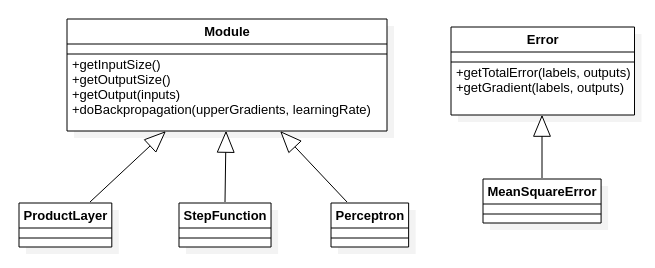
\includegraphics[width=0.7\linewidth]{images/UML.png}
			\caption{각 클래스의 관계를 UML로 표현한 그림. Module과 Error는 추상 클래스이다.}
		\end{figure}
	
		\begin{itemize}
			\item \textbf{ProductLayer}: $n$차원 벡터를 입력으로 받아서 $m$차원 벡터를 출력으로 내는 모듈로, 퍼셉트론에서 입력 벡터에 가중치들을 곱하여 출력 벡터를 만드는 과정과 동치이다. ($n$과 $m$은 객체의 생성자에서 할당할 수 있다.)
			\item \textbf{StepFunction}: 퍼셉트론을 위해 사용할 수 있는 활성화 함수로, 입력 값이 0보다 클 때만 출력으로 1, 그렇지 않으면 출력으로 0을 내는 함수이다.
			\item \textbf{Perceptron}: 본 과제에서 Logic gate를 학습시키는데 사용된다. 내부적으로 ProductLayer와 StepFunction을 멤버 변수로 가지고 있고, 입력값에 대한 출력값을 구하는 것은 ProductLayer와 StepFunction의 getOutput 함수를 순차적으로 호출하는 것으로 구현되고, Backpropagation 역시 역순으로 doBackpropagation 함수를 호출하는 것으로 구현된다.
			\item \textbf{MeanSquareError}: 평균 제곱 오차(Mean Square Error)에 따라 실제 정답($y_i$)과 네트워크가 예측한 출력값($\hat{y}_i$)과의 오류값을 계산한다.\\
			\[
			\text{MSE}=\frac{1}{N}\sum_{i=1}^{N} (y_i-\hat{y}_i)^2
			\]
		\end{itemize}
		
		위 UML의 관계와 같이 퍼셉트론의 각 과정을 클래스로 구현하여 모듈화함으로써, 각 클래스의 역할을 명확하게 구분할 수 있고, \textbf{퍼셉트론의 Backpropagation 과정을 각 Module 객체에 공통적으로 doBackpropagation 함수를 호출하는 것으로 매우 직관적으로 구현할 수 있다.}
	
	\subsection{소스 파일 구조}
	
		본 과제의 C++ 퍼셉트론 코드는 총 6개의 소스 파일로 구성된다.
		
		\begin{itemize}
			\item \textbf{Modules.h, Modules.cpp}: Perceptron을 구현하는데 필요한 각 모듈들을 클래스로 정의한다.
			\item \textbf{Perceptron.h, Perceptron.cpp}: Modules.h에서 정의한 모듈을 이용하여 Perceptron을 구현한다. 출력값을 구하는 과정과 역전파를 하는 과정 모두 각 모듈의 멤버 함수를 호출하는 것으로 구현된다.
			\item \textbf{Main.cpp}: AND, OR, XOR logic gate를 Perceptron 클래스를 이용하여 학습시킨다. 학습 후 결과(각 에폭 당 Error 값, 최종 진리표)를 CSV 파일로 저장한다. 추후 이 CSV 파일을 이용하여 학습 결과를 시각적으로 보여주는 그래프를 그린다.
			\item \textbf{Main.out}: 1.3.1에서 설명한 실행 환경에서 빌드한 실행 파일이다.
			\item \textbf{Makefile}: 소스 빌드 방법을 정의한 Makefile로, build-essential 패키지가 설치된 Linux 환경에서 ’make’ 명령어를 이용하여 빌드할 수 있다.
		\end{itemize}
	
	\section{실행 결과}
	
		\subsection{퍼셉트론 실행 환경}
	
			본 과제의 소스 코드는 Ubuntu 20.04 LTS (x86) 에서 개발 및 테스트 되었다. 순차적인 빌드 및 실행 방법은 아래와 같다.
			
			\begin{enumerate}
				\item Ubuntu 20.04 LTS와 같은 리눅스 환경에서 GCC를 이용하여 C++을 컴파일하기 위해 build-essential 패키지를 설치한다. (sudo apt install build-essential)
				\item 본 보고서와 함께 첨부된 소스 폴더(Makefile이 존재하는 디렉토리)에서 터미널을 실행하고, `make` 명령어를 실행한다.
				\item 빌드 결과 생성된 Main.out 파일을 실행한다.
			\end{enumerate}
		
		\subsection{퍼셉트론 실행 결과}
		
			위에서 설명한 실행 방법에 따라 퍼셉트론 학습 프로그램을 실행할 경우 아래와 같은 출력이 나타난다. 매 실행마다 랜덤 시드 값이 재설정되므로 정확한 출력은 다를 수 있으나, XOR 게이트는 끝까지 학습되지 않는다는 점은 항상 같다.
			
			그리고 프로그램이 완료되면 \textbf{results}라는 이름의 서브 디렉토리에 학습 결과가 CSV 파일로 저장된다.
			
			\begin{minted}
				[
				frame=lines,
				framesep=2mm,
				baselinestretch=1.2,
				fontsize=\footnotesize,
				linenos
				]
				{text}
Trainning AND Gate...
- Epoch #1 MSE: 2
- Epoch #2 MSE: 3
- Epoch #3 MSE: 2
- Epoch #4 MSE: 2
- Epoch #5 MSE: 3
- Epoch #6 MSE: 2
- Epoch #7 MSE: 1
- Epoch #8 MSE: 0
Successfully trained AND Gate!
* Saved result files(./results/*.csv).

Trainning OR Gate...
- Epoch #1 MSE: 1
- Epoch #2 MSE: 2
- Epoch #3 MSE: 1
- Epoch #4 MSE: 0
Successfully trained OR Gate!
* Saved result files(./results/*.csv).

Trainning XOR Gate...
- Epoch #1 MSE: 2
- Epoch #2 MSE: 4
- Epoch #3 MSE: 4
- Epoch #4 MSE: 4
- Epoch #5 MSE: 4
- Epoch #6 MSE: 4
- Epoch #7 MSE: 4
- Epoch #8 MSE: 4
- Epoch #9 MSE: 4
- Epoch #10 MSE: 4
- Epoch #11 MSE: 4
- Epoch #12 MSE: 4
Failed to train XOR Gate...
* Saved result files(./results/*.csv).
			\end{minted}
		
		\subsection{학습 결과 그래프}
		
			이전에 소개한 퍼셉트론 학습 프로그램에서 학습 후 생성하는 결과 CSV 파일을 그래프로 그리는데 plot-results.py 스크립트를 사용할 수 있다. 스크립트를 실행하기 위해서는 matplotlib, numpy 패키지가 설치된 Python 3 인터프리터가 필요하다.
			
			퍼셉트론 학습 프로그램에서 CSV 파일을 생성한 뒤 plot-results.py를 실행하면 다음과 같은 결과를 확인할 수 있다. 아래 그림에서 확인할 수 있듯이 AND와 OR 게이트는 빠르게 학습되어 MSE가 감소하는 그래프를 보여주지만 XOR은 MSE가 감소하지 못하고 12번의 iteration을 거친 후에도 틀린 결과를 내놓았다. 이는 단순한 1층 퍼셉트론으로는 XOR을 학습시킬 수 없다는 사실을 시사한다.
			
			\begin{figure}[h]
				\centering
				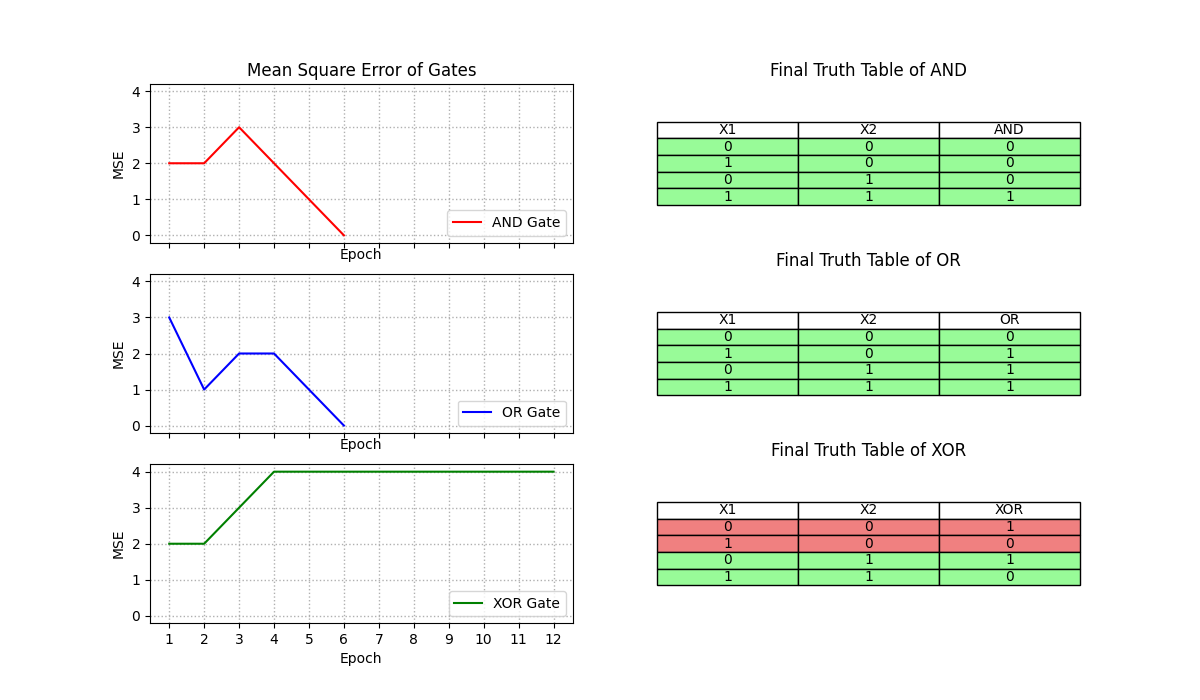
\includegraphics[width=0.9\linewidth]{images/Figure_1.png}
				\caption{퍼셉트론 학습 결과를 Python 스크립트로 그린 그림. 좌측은 AND, OR, XOR 게이트를 학습하는 과정에서 각 에폭마다 측정한 MSE, 우측은 학습이 끝까지 진행되고 나서 작성한 진리표이다.}
			\end{figure}
			
			
	
\end{document}
